%\documentclass[11pt]{amsart}
\documentclass[11pt]{scrartcl}
\usepackage{geometry}
\geometry{letterpaper}
\usepackage{graphicx}
\usepackage{amssymb}
\usepackage{epstopdf}
\usepackage{listings}
\usepackage{color}
\usepackage{booktabs}
\DeclareGraphicsRule{.tif}{png}{.png}{`convert #1 `dirname #1`/`basename #1 .tif`.png}
\title{Similar Days at Airports in the New York Area}
\author{Akhil Shah, Kenneth Kuhn, Chris Skeels}
%\date{}
\begin{document}
\maketitle


\section*{Executive Summary}

Note that the 

\begin{itemize}
\item why cluster similar days? analysis of tfmi must account for conditions, which this 
helps 
\item web-based app - helps users explore and visualize clusters.  We use k-means and DBSCAN
\item use observed and forecasted weather/traffic features, mostly selected by expert judgement.  Also used PCA.
\item list of data sources that were used
\item results depend on \{feature selection methodology, clustering algo, and data\}.  little evidence days are arranged in clusters.  but we provide guidance on selecting a triplicate based on how the results of the analysis are to be used.
\end{itemize}
The primary purpose of this phase of our study was to investigate various methodologies for clustering similar days using Airport level data.  We have derived clusters of similar days using the following sequence of steps: selecting data feature upon which to cluster, the clustering algorithm, and the method by which to choose the algorithmic parameters.  Each of the various methodologies we have explored is thus distinguished by the choice made in each of those steps.  In the table below we summarize our choices for each of these options

\begin{table}[htdp]
\caption{default}
\begin{center}
\begin{tabular}{|c|c|c|}
Option & Feature selection & Clustering Algorithm\\
\hline 
1 & Knowledge based & K-means\\
2 & Traffic Biasing & K-means\\ 
3 & Temporal PCA & K-means\\ 
2 & Traffic Biasing & DBSCAN\\ 
\end{tabular}
\end{center}
\label{default}
\end{table}%

It is important to note that the dominant factor which determines the quality of any machine learning (or more generally, statistical model) approach is the selection of features that are most relevant rather than the choice of prediction or clustering algorithms.  Generally, the best source for relevant features are derived from expert domain knowledge.  However machine learning methods for feature selection can complement such expert elicitation by quantifying the relevance of each feature.  Moreover feature selection methods usually rely on having a dataset with accompanying ground truth labels.  For example, if we were interested in determining which weather and traffic features were most relevant to predicting a Ground Delay Program (GDP) on any given day, the feature selection algorithm would require a ``training" dataset that included not only the predictors (weather and traffic) but also the observed ground-truth label of absence or presence of GDP for each data record \cite{mukherjeepredicting}.  The goals of this algorithm would be to model current GDP decision making and/or to forecast future GDP decisions.  Our goal was somewhat different, to explore, characterize, and categorize airport weather and traffic conditions without modeling current GDP decision making.  Therefore, it was not appropriate, for our study, to use any sort of ground-truth labels.  The lack of ground-truth labels rules out various feature selection methods \cite{guyon2003introduction}.  Methods for feature selection and cluster analysis in an `unsupervised' environment like ours are often based on finding the most clearly defined clusters possible.  While we are interested in finding clearly defined clusters, where possible, we are most interested in identifying features that summarize and characterize how analysts and air traffic control planners describe airport weather and air traffic at airports\dots


\section*{Introduction and Context}
Personnel at the Federal Aviation Administration's Air Traffic Control System Command Center and at airline operations centers regularly implement Air Traffic Flow Management Initiatives (ATFMIs) purposefully delaying, canceling, and rerouting flights. These initiatives increase the safety and efficiency of the nation�s air transportation system, for example by replacing airborne delay with ground delay, and are necessary during inclement weather and in other situations where demand for system resources exceeds capacity.  In particular, problems at airports often create the need for ATFMIs.  Analysis of the past use of ATFMIs can demonstrate the relative success of courses of action but must account for the distinct conditions faced during planning and operations.  An identification of days that are similar can help, for example allowing analysts to focus on the 10 days in the past two years when there was thunderstorm activity at the key airports in the New York area between 8am and 11am, local time, but clear weather the rest of the day.

This report describes our work to develop methodologies for the identification similar days in terms of aviation weather and air traffic operations at the airports in the New York area.  There are many reasons why an analyst may want to identify similar days and thus there are multiple ways to arrive at a definition of similar days.  This report follows an earlier report to identify similar days based on conditions in the airspace around New York City.  We do not wish to replicate the prior report and thus only report on new findings specific to our study of airports.  The earlier report includes more detail regarding why it would be beneficial to identify similar days from the perspective of ATFMI planning or operations.

As in our earlier work that focused on the airspace, we have published many of our results focusing on airports in a web based application.  The application is essentially identical to the one we developed and reported on previously.  Please see the earlier report for a description of our web based application.

In this report, we report on our work to identify features that describe aviation weather and air traffic at airports in the New York area, the data sets we use to define these features, and interesting results we obtain.  The final section of this report is a conclusion that details how the airport-focused results presented here can be blended with airspace-focused results obtained previously.

\section*{Selecting Features to Describe Airport Conditions}
Our clustering results were derived from features that were selected by either surveying the literature for those considered relevant or using heuristics.  In the sections below we summarize the literature employed for knowledge-based feature selection and also our heuristic methodologies: Traffic Biasing and Temporal PCA, both of which reduce the 24 hourly observations of airport weather and traffic data to a single observation per day.  
\subsection*{Knowledge-Based Feature Selection}
Previous studies have employed airport-centric observations and forecasts of weather and traffic data for clustering similar days.  We will use these weather and traffic features identified as `relevant' as part of our overall clustering analysis, and consider the feautres use to derive the clusters as selected by ``expert judgement."  Below we summarize  and our subsequent application of them in clustering similar days from an airport perspective.  In these studies, features are initially identified based on domain knowledge, and then filtered for relevancy using either correlation analysis or other statistical measures, when used as explanatory varaibles in a statistical model for predicting the observed TFM data \cite{mukherjeepredicting,grabbe2013similar}.  

In \cite{mukherjeepredicting}, the authors employ logistic regression and decision trees to predict the absence or presence of GDP every hour at EWR.  Expanatory variables which are determined as statistically significant as predictors include: demand capacity ratio and queueing delay, derived from hourly scheduled arrival data in ASPM and the assumed arrival capacity from Capacity Benchmark report; and meteorlogical data including the present hours visibility and WITI index for the New York Center (ZNY), and average over the previous three hours of wind speed, demand capacity ratio and WITI of ZNY.  These seven features were determined to be statistically significant as predictors of hourly GDP at EWR, whereas cloud ceiling and cross-winds at EWR were deemed to be not.  

In \cite{grabbe2013similar} the authors performed clustering of EWR airport-level data which included observed hourly arrivals and hourly wind speed, wind gusts, wind direction, and ceiling.  These features were selected as relevant by performing a correlation analysis with the absence or presence of hourly GDP at EWR.  Note unlike the previous analysis, visibility at EWR was determined to be not as strong a predictor of GDP, and thus was not used in their subsequent clustering\footnote{Textural descriptions of precipitation were also presumably ruled out as relevant and thus not employed in their clustering analysis.}

As an alternative to generating clusters of days, the authors of \cite{liu2014} employ a semi-supervised  method to identify similar days to a given day using a distance metric applied to hourly forecasted weather data on those days at a given airport (using TAF data).  One of their main contributions is to derive a distance metric from user supplied specifications of similarity and dissimilarity between various hours in the dataset, using runway configurations, Airport Acceptance Rates (AAR), and Meteorological conditions (MC).  The derived (learned from data and user supplied specifications) metric minimizes the distance between weather feature vectors at hours that are defined to be similar, while ensuring the distance between feature vectors at dissimilar hours is greater than one. Employing such a semi-supervised distance metric, their proof-of-concept example selects two days in 2012 at EWR and using a distance metrics, learned from similar and dissimilar hourly specifications for 2011 TAF and ASPM data, derives the five most similar days from 2011 to each of the two given 2012 days.  Their feature vector is nine-dimensional and consist of boolean values for absence/presence of thunderstorm and snow, and various functional transformations of visibility, ceiling and wind speed

Our clustering analysis of the NY metro region we will use \emph{some} of the features identified as relevant by \cite{mukherjeepredicting} using airport data at EWR, JFK, and LGA. As we only had access to ASPM and METAR data, we will reduce the 24 hourly observations for each day into 8 3-hour averages for each of the following features: scheduled arrivals, visibility, and wind-speed.
 
\subsection*{Traffic Biasing}
Both our weather and traffic datasets contain multiple hourly observations per day.  Since we are interested in exploring similar days, feature selection includes not only selecting particular observed or forecasted variable but also at which hour or hours.  At the extremes, one could decide to use all of the hours for any variable as separate feature, which would certainly encroach the curse of dimensionality, or select a single point in time, which would incur a loss of information penalty.  A reasonable compromise might be to uniformly average the values of numerical variables over the 24 hourly observations to produce a single value for a given day.  However we employ a weighted average, the weight of which are determined through the following heuristic: determine daily average arrival count for a given airport, and normalize these counts to sum to one.  In our case we used ASPM arrival counts from 2010-2013 to determine the average hourly arrival for each of the three New York region airports in our analysis.  Once normalized, these form 24 weights $w_h$, where $h$ is the hour index, and are then used to form the weighted average for the METAR numerical variables.  For example, a given day's visibility at JFK would have the following expression to reduce the 24 observed values to a single value $v^{TB}_{d} = \sum_{h}^{24} w_h v_{dh}$, where $d$ is the index for a given day in the dataset.   

Below we show the hourly variation of arrival data at JFK for every day between 2010-2013.  Note there is a clear pattern for traffic, and as expected, some hours are much busier than others.  Thus the Traffic Biasing heuristic serves to select the temporal dependence of features which will be used for subsequent clustering.  

\emph{insert box plot of hourly arrivals at JFK here}


\subsection*{Temporal PCA}
Another heuristic we have explored for feature selection is based on PCA, and similar to Traffic Biasing, serves to shape the temporal dependence of an observed or forecasted variable from the weather and traffic datasets.  In this scheme, a single variable, say visibility at JFK for a given date, is reduced to a single value for that day using PCA to select the linear combination 24 observed values which captures the largest variation (i.e. the first PCA component).  

Below we show the first three PCA components of a given day at JFK for various weather variables in the METAR dataset.  Note that some variables do have strongly explanatory first PCA component, but others do not.  As a result, we will postpone further integration of this heuristic into our clustering analysis until we can quantitatively asses the relevance of such features in a more principled feature selection framework (i.e. with TFMI data serving as ground-truth labels).

\emph{insert box plot of hourly arrivals at JFK here}


\section*{Airport Weather and Air Traffic Data}
We spit the types of data of interest into data that describe conditions at airports versus in the airspace, as well as those that describe weather versus those that describe scheduled operations.

Airports themselves issue Terminal Area/Aerodrome Forecast reports (TAFs) and Aviation Routine Weather Reports (METARs) which summarize local forecast and observed weather conditions. METARs can contain select forecast data but, generally speaking, TAF data are forecast data while METAR data are observational data. TAF and METAR data contain information on: wind speed and direction, wind gusts, visibility, precipitation, cloud height, cloud cover, humidity, and pressure. Prior research efforts have linked many of these variables to traffic flow management initiatives. Previous studies \cite{smith2009decision} have  successfully used TAF data to forecast Ground Delay Program initiation, but without giving details on the relative importance of specific variables.  The authors in \cite{mukherjeepredicting} point out the relevance of hourly observations of visibility, cloud height, wind, convection, and precipitation in particular, again for predicting GDPs. TAFs and METARs are issued roughly hourly to ensure reports keep up with changing weather conditions but also that distinct consumers of the data have a consistent report and time to plan against it.  A related study \cite{wolfe2011method} analyzed combinations of features (``queries") from airport-specific Weather Impacted Traffic Index (WITI) data to determine which were most relevant in predicting observed weather-related GDP from present time to six hours in the future.  They developed an information-retrieval model consisting of thresholding WITI features as queries or rules.  Their model was trained using observed 2008 GDP data, as recorded in the National Traffic Management Log (NTML), and tested on 2009 GDP data.  However this study concluded that the rules based on WITI features were only slightly more predictive than a constant rule which always predicted ``no GDP'. 

The studies cited above, along with \cite{liu2014} focus on forecasts, typically forecast conditions two hours ahead of time. Different TFMIs are implemented at different time scales, e.g., flow metering is typically used to respond to short-term supply-capacity imbalances while Ground Delay Programs are used to mitigate the potential for a larger problem further in the future. It is not obvious that two-hour forecast data is the ideal for our efforts. There is actually a larger question as to the relative importance of differences between weather forecast and observational data here. When determining that January 1, 2012 is similar to January 2, 2012 but not to July 1, 2012, it may or may not matter a great deal whether forecast or observed weather data are used. DeLaura and Allan (2003) show how, for analyses they perform, differences between forecast and observed weather patterns are relatively unimportant. Their conclusion is that, for air traffic flow management tools, a realistic operational model may be at least as important as the frequently discussed problem of weather forecast uncertainty. This is a somewhat surprising statement given that the authors are concerned with route guidance, where small details can be important. We do note that the authors do not claim that forecast uncertainty is completely unimportant.

For now, we note that a collection of hourly observations of TAF and METAR data, or other data detailing the variables included in TAF and METAR data, covering the busiest airports in the New York area over an extended period of time would comprise an ideal data set to describe airport weather in the area at the time.

Traffic flow management is concerned with mitigating temporary supply and demand imbalances. At the level of an airport, the primary concern is almost always that the number of aircraft scheduled to land at and take off across a set block of time may be higher than the throughput of the runways will allow. A reasonable length for such a block of time would be an hour or a few hours. Supply-demand imbalances over shorter periods of time, e.g., two aircraft scheduled to land at the same time, can be accommodated with minor path adjustments rather than the more strategic traffic flow management initiatives. Hourly observations of scheduled operations could be easily compared to weather data such as TAFs and METARs that are reported hourly. A collection of hourly observations of the numbers of aircraft scheduled to land at and take off from the busiest airports in the New York area would be an ideal data set here.

Our definition of the ideal data set for describing airport weather referenced TAFs and METARs, two formats airports currently use in their reports. Current TAF and current METAR data are available. METAR data has been collected in a publicly accessible historical archive. Unfortunately, we have not identified a similar large archive of historical TAF data. This result is unsurprising; there are relatively many uses for historical observations of weather conditions and relatively few for historical forecasts. Luckily, there is an alternate data source that does contain both forecast and observed weather at airports. The National Oceanic and Atmospheric Administration's (NOAAs) Localized Aviation MOS (Model Output Statistics) Product (LAMP) combines much of the same data that appears in TAF and METAR data. This data is free to download from NOAA. Table 1 summarizes the availability of useful airport weather data.

\begin{table}[htdp]
\caption{Summary of Airport Data}
\begin{center}
\begin{tabular}{|c|c||c|}
Name & Feature & Notes

\end{tabular}
\end{center}
\label{default}
\end{table}%

\subsection*{LAMP Data details}
An overview of LAMP can be found in \cite{ghirardelli2005overview}.  In summary, the LAMP forecasting model runs hourly and goes out to 25 hours for CONUS, Hawaii, Alaska and Puerto Rico.  For data sources it uses both surface observations and radar data.  The main premise of LAMP is that most recent surface obs (mostly METAR reports, used as reported after undergoing quality control checks) can have strong predictive value in updating MOS. Radar data (16-level 2km WSI and 7-level 10km RCM) used as predictors for thunderstorm development.  Observed lightning from National Lightning Detection Network used in development of thunderstorm probabilities. 

The following are forecasted by LAMP:
\begin{itemize}
\item{Prob. of precipitation $>$ 0.01 inches in 6 or 12h period}
\item{Precipitation type (liquid, snow, freezing) conditional on precipitation occurring}
\item{Probability of ceiling height belonging to a fixed set of altitudes}
\item{Probability of total sky cover belonging to a fixed set of categories (e.g. clear, few, overcast, etc.)}
\item{Probability of visibility belonging to a fixed set of ranges}
\item{Probability of obstruction to vision belonging to a fixed set of categories (e.g. haze, mist, fog, etc.)}
\item{Probability of thunderstorm in 2h bins (for 25h out since start of LAMP run)}
\end{itemize}

\subsection*{METAR data details}
Metar features are observed hourly: temperature, dew point, humidity, sea-level pressure, visibility, wind direction, wind speed, gust speed, precipitation, condition code, event code.  


\section*{Results and Discussion}
\subsection*{Exploratory Analysis}
Below we summarize the statistical variation of the datasets we have used to derive features and cluster days.  

Variation over 24 hours of selected METAR weather variables for days in 2010-2013.
%%--graphics here-%%%
\begin{figure}[htbp]
\begin{center}

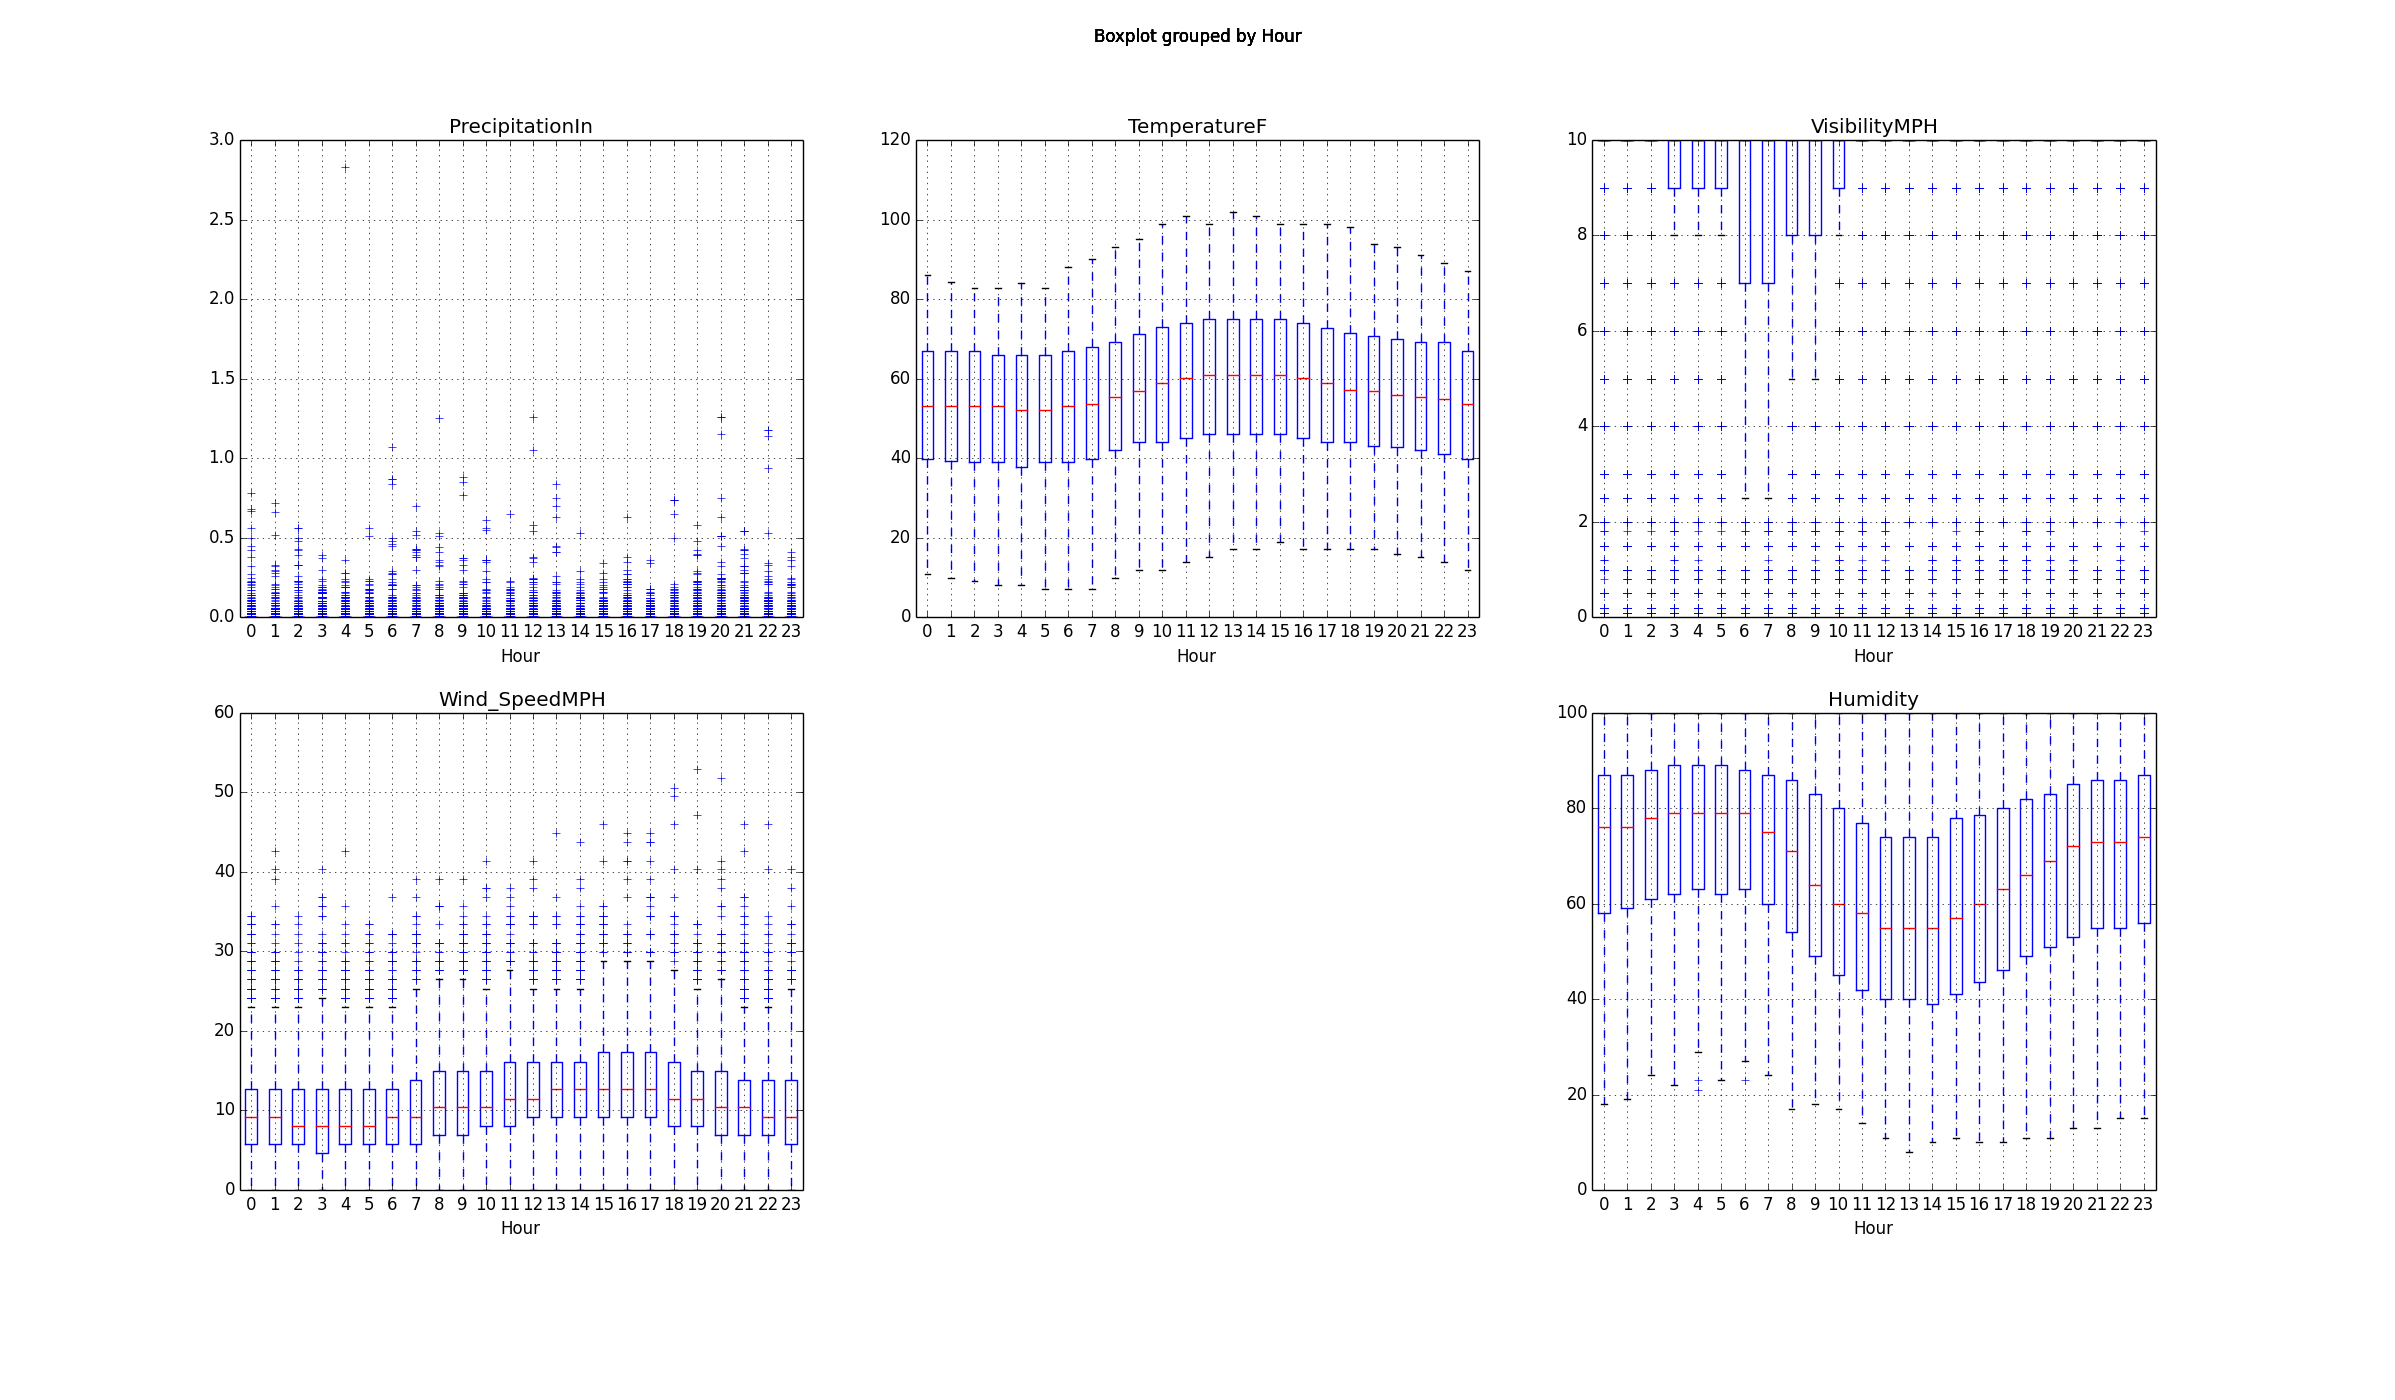
\includegraphics[scale=0.25]{./figures/boxplot_hourlyvariation.png}

\caption{JFK - annual exploratory statistics of METAR data}
\label{default}
\end{center}
\end{figure}

Variation over years of selected METAR weather variables every year.  
%%--graphics here-%%%
\begin{figure}[htbp]
\begin{center}

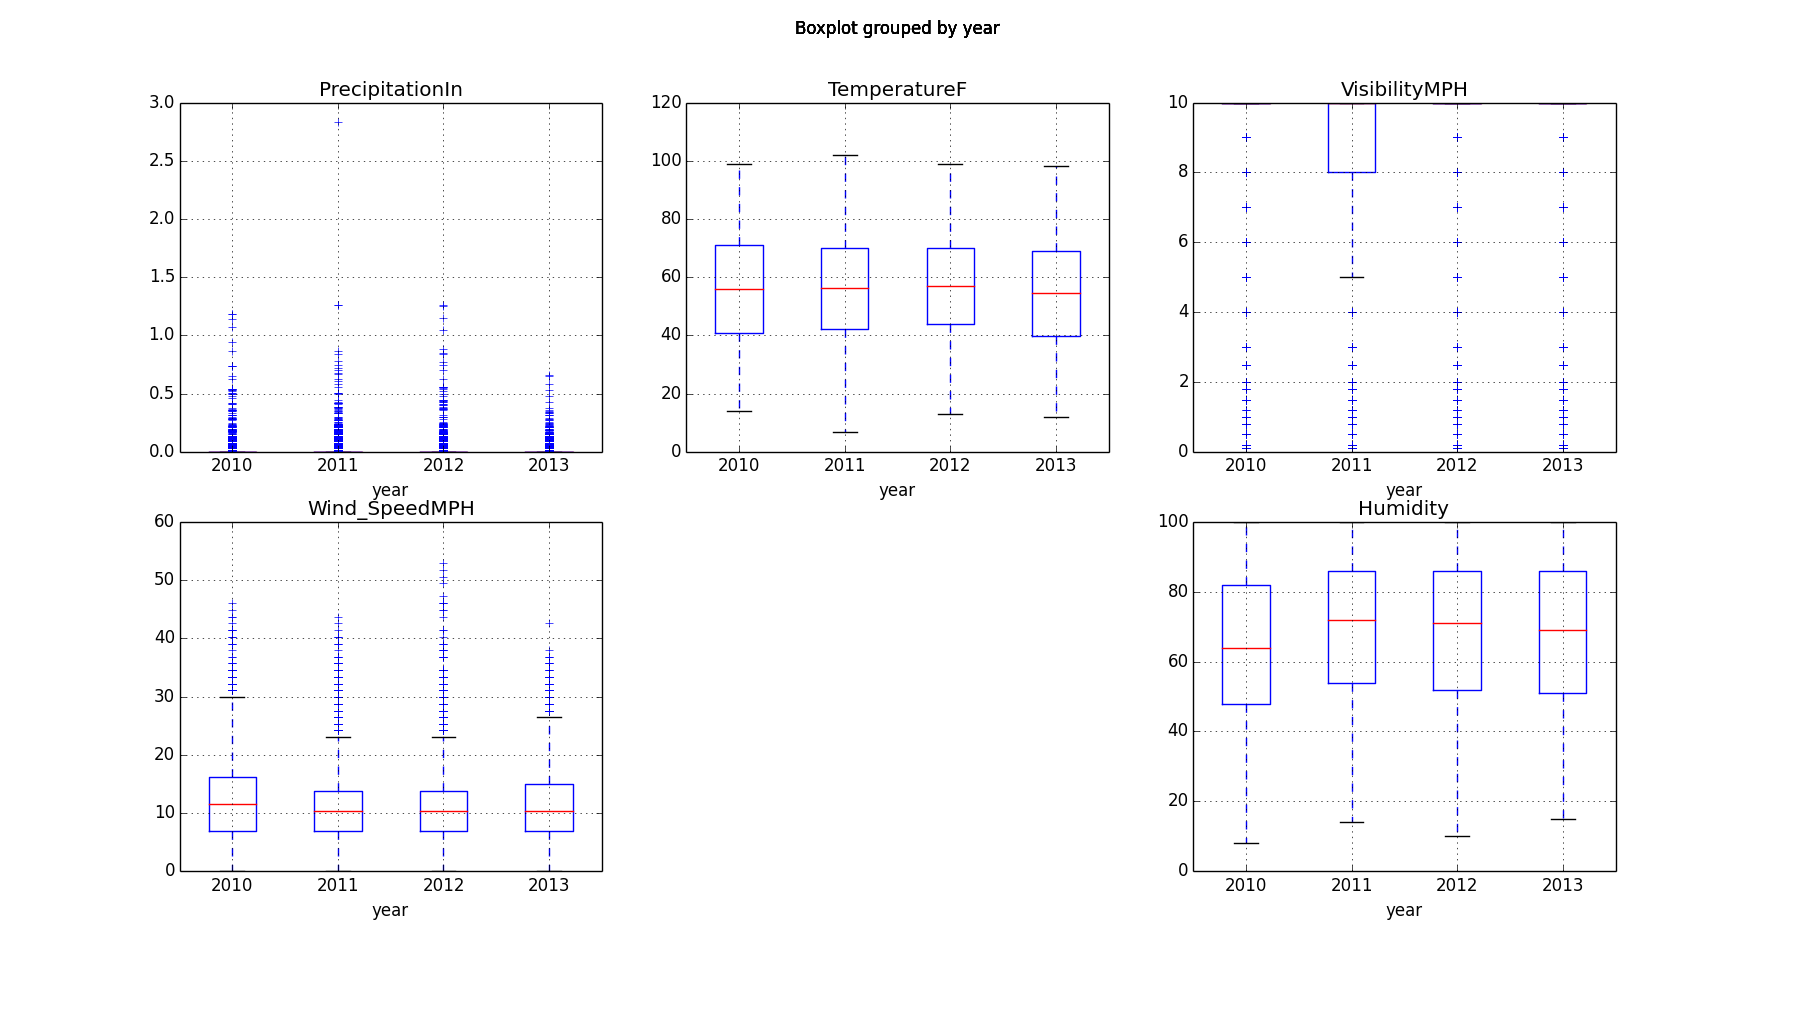
\includegraphics[scale=0.35]{./figures/boxplot_annualvariation.png}

\caption{JFK - annual exploratory statistics of METAR data}
\label{default}
\end{center}
\end{figure}




%%%concurrency table
\subsection*{Assessing Clusters}
When ground-truth labels are available, clusters can be assessed by various quantitative metrics that characterize the intra-cluster similarity of those labels versus the inter-cluster similarity of labels.  One example of such a metric is the RAND index, but there are various others.  More generally a ``confusion matrix" is a standard representation in Machine Learning to present the accuracy of an algorithm that models a categorial variable.  Typically, a model that has been fit using a training data set is asked to forecast the categorical variable in a distinct test data set.  The rows of the confusion matrix represent the actual values of the categorical variable in the test data set while the columns represent the model output values of the categorical variable using the model inputs from the test data set.  Each cell in the matrix is a count showing how many times the model predicted label x (column) when the actual observation was was label y (row).

Although there are proposals for selecting features without ground-truth labels, they rely on having an underlying statistical model for the joint distribution of predictors and prediticand \cite{cai2010unsupervised,Roth04featureselection}.  An alternative approach may be to cull a given set of features until an optimal clustering quality criterion (e.g. Silouhette width) is achieved.  However such a combinatorial optimization would grow exponentially with the dimension of the feature space, which can be quite large for even if we restrict ourselves to only ASPM arrival and departure data (24 observations/day $\times$  (11 METAR + 2 ASPM) $\times$ 3 Airports in the NY region).  Hence such a combinatorial optimization approach is likely infeasible and moreover may not yield features that adequately characterize how expert and planners conceive of days, which is our primary goal. Instead in this phase we have applied heuristic methods described in the above table, such as Traffic biasing, which employs some domain knowledge in reducing the 24 observations per day using a weighted average derived from the historical hourly arrival rates at each airport. 

Although we do not wish to optimize measures of intra-cluster versus inter-cluster similarity such as the Silhouette score, we are still interested in such scores.  If the data are numeric this metric can be computed for each sample using for example the euclidean distance metric\footnote{If the clustering algorithm used a distance measure, rather than a similarity matrix to assign the clusters in the first place, it is more natural to use the same distance metric in computing the Silhouette score}.  

In addition, we propose a novel method to use categorical data as ``psuedo-labels" for each observation.  The data we use for these psuedo-labels are the observed ``Condition" data column of METAR data, a categorical value.  Each day (sample of our data-matrix) has 24 such values and we propose three types of concurrency tables which allow use to analyze the similarity within and between the clusters using the frequency of occurrence of those categorical values.
\subsection*{Concurrency Tables}
The Condition data within METAR data describe weather conditions at an airport using a categorical variable.  The data are not ground-truth labels in the sense that we would explicitly seek to build a model of this data or claim that the data adequately summarize airport weather data for air traffic flow management initiative planning.  However, it is worthwhile to compare the results of cluster analysis to the Condition data, to see if, for example, days with the Condition label of ``Thunderstorm'' appear in one cluster while days with the Condition label of ``Clear'' appear in another cluster.  To explore the relationship between the METAR Condition data and identified clusters, we created concurrency tables.  The idea is similar to that of the Confusion Matrix described above.  Each row in a concurrency table refers to a specific Condition label and each column to a specific cluster output by a clustering algorithm.  Each cell in a concurrency table contains a count of the number of times a day was assigned to a specific Condition label (row) according to observed METAR data and a specific cluster (column) according to the results of a specific form of cluster analysis.

%Using results from:
%/Users/ashah/NoBackup/code/nasa/results/JFKexpert_kmeans_5.csv

Day-Aggregrated counts:
\begin{tabular}{lrrrrr}
\toprule
{} &     1 &     2 &     3 &      4 &      5 \\
\midrule
Blowing Snow                  &   NaN &   NaN &   NaN &      2 &      2 \\
Clear                         &   490 &   548 &  1936 &   2651 &   2674 \\
Fog                           &     5 &   230 &   233 &    238 &    462 \\
Haze                          &    55 &   181 &   202 &    207 &    310 \\
Heavy Rain                    &    22 &    74 &    80 &    155 &    238 \\
Heavy Snow                    &   NaN &     4 &     4 &      6 &     24 \\
Heavy Thunderstorms and Rain  &    36 &    62 &    66 &     71 &     86 \\
Ice Pellets                   &   NaN &     3 &     3 &      5 &      6 \\
Light Drizzle                 &     9 &   144 &   170 &    191 &    458 \\
Light Freezing Drizzle        &   NaN &     7 &     7 &      7 &     45 \\
Light Freezing Rain           &   NaN &     4 &     4 &      4 &     36 \\
Light Ice Pellets             &   NaN &     3 &     4 &      4 &     24 \\
Light Rain                    &   347 &   874 &  1330 &   1867 &   2799 \\
Light Rain Showers            &   NaN &   NaN &   NaN &      1 &      1 \\
Light Snow                    &   NaN &   194 &   304 &    463 &    814 \\
Light Thunderstorms and Rain  &    70 &   100 &   123 &    128 &    146 \\
Light Thunderstorms and Snow  &   NaN &   NaN &   NaN &    NaN &      1 \\
Mist                          &   NaN &    12 &    12 &     12 &     27 \\
Mostly Cloudy                 &  3410 &  4483 &  8639 &  11069 &  11501 \\
Overcast                      &  1135 &  2319 &  4619 &   5825 &   7271 \\
Partly Cloudy                 &   950 &  1075 &  2924 &   4404 &   4455 \\
Patches of Fog                &   NaN &     4 &     4 &      4 &      5 \\
Rain                          &    40 &   150 &   184 &    264 &    481 \\
Scattered Clouds              &  2068 &  2448 &  4859 &   6562 &   6659 \\
Shallow Fog                   &     2 &     2 &     2 &      2 &      2 \\
Smoke                         &   NaN &   NaN &     1 &      1 &      1 \\
Snow                          &   NaN &    15 &    18 &     40 &     71 \\
Squalls                       &   NaN &   NaN &     1 &      1 &      1 \\
Thunderstorm                  &    47 &    51 &    62 &     67 &     68 \\
Thunderstorms and Rain        &    24 &    35 &    40 &     47 &     53 \\
Thunderstorms with Small Hail &   NaN &     1 &     1 &      1 &      1 \\
Unknown                       &     5 &     7 &    11 &     16 &     20 \\
\bottomrule
\end{tabular}


Day-Most frequent counts:
\begin{tabular}{lrrrrr}
\toprule
{} &     1 &     2 &     3 &     4 &     5 \\
\midrule
Clear                  &   117 &   117 &   655 &   899 &   899 \\
Fog                    &   NaN &    72 &    72 &    72 &   132 \\
Haze                   &   NaN &    10 &    10 &    10 &    33 \\
Heavy Rain             &   NaN &   NaN &   NaN &    25 &    25 \\
Light Drizzle          &   NaN &    20 &    20 &    20 &    54 \\
Light Freezing Drizzle &   NaN &   NaN &   NaN &   NaN &    23 \\
Light Rain             &    48 &   282 &   397 &   566 &  1112 \\
Light Snow             &   NaN &   147 &   196 &   262 &   551 \\
Mostly Cloudy          &  2616 &  3205 &  6215 &  7825 &  7903 \\
Overcast               &   453 &  1181 &  2337 &  2885 &  3837 \\
Partly Cloudy          &   334 &   358 &  1146 &  1837 &  1837 \\
Rain                   &   NaN &     9 &     9 &     9 &     9 \\
Scattered Clouds       &  1113 &  1186 &  2126 &  2828 &  2852 \\
Snow                   &   NaN &   NaN &   NaN &    12 &    22 \\
\bottomrule
\end{tabular}


Day-Least frequent counts:
\begin{tabular}{lrrrrr}
\toprule
{} &    1 &    2 &    3 &    4 &    5 \\
\midrule
Clear                        &   73 &   79 &  252 &  343 &  348 \\
Fog                          &  NaN &   12 &   12 &   13 &   17 \\
Haze                         &   11 &   22 &   35 &   38 &   48 \\
Heavy Rain                   &    4 &   22 &   25 &   35 &   60 \\
Heavy Snow                   &  NaN &    4 &    4 &    4 &    4 \\
Heavy Thunderstorms and Rain &    5 &    7 &    7 &    9 &   14 \\
Ice Pellets                  &  NaN &  NaN &  NaN &  NaN &    1 \\
Light Drizzle                &    1 &   14 &   23 &   30 &   66 \\
Light Freezing Drizzle       &  NaN &  NaN &  NaN &  NaN &    2 \\
Light Freezing Rain          &  NaN &  NaN &  NaN &  NaN &    1 \\
Light Ice Pellets            &  NaN &    1 &    2 &    2 &    7 \\
Light Rain                   &   50 &   76 &  150 &  205 &  220 \\
Light Rain Showers           &  NaN &  NaN &  NaN &    1 &    1 \\
Light Snow                   &  NaN &    3 &    6 &   26 &   27 \\
Light Thunderstorms and Rain &   18 &   22 &   28 &   30 &   30 \\
Light Thunderstorms and Snow &  NaN &  NaN &  NaN &  NaN &    1 \\
Mist                         &  NaN &   10 &   10 &   10 &   14 \\
Mostly Cloudy                &  141 &  158 &  366 &  508 &  534 \\
Overcast                     &   94 &  109 &  281 &  383 &  397 \\
Partly Cloudy                &  189 &  206 &  486 &  661 &  665 \\
Patches of Fog               &  NaN &  NaN &  NaN &  NaN &    1 \\
Rain                         &   15 &   29 &   40 &   60 &   90 \\
Scattered Clouds             &  178 &  198 &  603 &  752 &  769 \\
Shallow Fog                  &    2 &    2 &    2 &    2 &    2 \\
Smoke                        &  NaN &  NaN &    1 &    1 &    1 \\
Snow                         &  NaN &  NaN &  NaN &  NaN &    3 \\
Squalls                      &  NaN &  NaN &    1 &    1 &    1 \\
Thunderstorm                 &    3 &    5 &    5 &    5 &    5 \\
Thunderstorms and Rain       &   10 &   18 &   19 &   22 &   27 \\
Unknown                      &    1 &    2 &    4 &    4 &    6 \\
\bottomrule
\end{tabular}


Condition Concurrency Tables for airport:EWR

%Using results from:
%/Users/ashah/NoBackup/code/nasa/results/EWRexpert_kmeans_5.csv

Day-Aggregrated counts:
\begin{tabular}{lrrrrr}
\toprule
{} &     1 &     2 &     3 &     4 &      5 \\
\midrule
Blowing Snow                        &   NaN &   NaN &    10 &    10 &     10 \\
Clear                               &   516 &  1446 &  1514 &  1546 &   3176 \\
Fog                                 &   NaN &   NaN &    70 &   147 &    149 \\
Haze                                &    29 &    35 &   191 &   416 &    525 \\
Heavy Ice Pellets                   &   NaN &   NaN &   NaN &     1 &      1 \\
Heavy Rain                          &     5 &    20 &    90 &   242 &    284 \\
Heavy Snow                          &   NaN &     1 &    18 &    53 &     53 \\
Heavy Thunderstorms and Rain        &     3 &    15 &    31 &    56 &    128 \\
Ice Pellets                         &   NaN &   NaN &     3 &    12 &     12 \\
Light Drizzle                       &     4 &    25 &   158 &   618 &    656 \\
Light Freezing Drizzle              &   NaN &   NaN &     7 &    48 &     48 \\
Light Freezing Rain                 &   NaN &   NaN &    17 &    52 &     52 \\
Light Ice Pellets                   &     3 &     8 &    14 &    39 &     41 \\
Light Rain                          &   151 &   547 &  1217 &  2633 &   3438 \\
Light Rain Showers                  &   NaN &   NaN &   NaN &     1 &      1 \\
Light Snow                          &    45 &   143 &   434 &   834 &    881 \\
Light Thunderstorms and Ice Pellets &   NaN &   NaN &   NaN &     2 &      2 \\
Light Thunderstorms and Rain        &     3 &    32 &    54 &    88 &    199 \\
Mist                                &   NaN &   NaN &   NaN &     3 &      3 \\
Mostly Cloudy                       &  1634 &  4074 &  5015 &  5404 &  11420 \\
Overcast                            &   886 &  2021 &  3168 &  4695 &   7838 \\
Partly Cloudy                       &   551 &  1833 &  1947 &  1988 &   3679 \\
Rain                                &     4 &    60 &   182 &   492 &    560 \\
Scattered Clouds                    &   881 &  2537 &  2835 &  2932 &   5746 \\
Smoke                               &   NaN &   NaN &   NaN &   NaN &      1 \\
Snow                                &     6 &    11 &    41 &    91 &     91 \\
Thunderstorm                        &     5 &    27 &    44 &    47 &    121 \\
Thunderstorms and Rain              &     4 &    17 &    30 &    55 &     94 \\
Unknown                             &     4 &    12 &    14 &    15 &     17 \\
\bottomrule
\end{tabular}
Day-Most frequent counts:
\begin{tabular}{lrrrrr}
\toprule
{} &     1 &     2 &     3 &     4 &     5 \\
\midrule
Blowing Snow           &   NaN &   NaN &     9 &     9 &     9 \\
Clear                  &   225 &   613 &   613 &   613 &  1235 \\
Fog                    &   NaN &   NaN &    10 &    32 &    32 \\
Haze                   &     8 &     8 &    40 &   118 &   137 \\
Heavy Rain             &   NaN &   NaN &    15 &    15 &    15 \\
Heavy Snow             &   NaN &   NaN &   NaN &    17 &    17 \\
Light Drizzle          &   NaN &   NaN &    11 &   152 &   152 \\
Light Freezing Drizzle &   NaN &   NaN &   NaN &    25 &    25 \\
Light Freezing Rain    &   NaN &   NaN &    10 &    10 &    10 \\
Light Rain             &    17 &   146 &   485 &  1457 &  1594 \\
Light Snow             &    14 &    51 &   295 &   627 &   639 \\
Mostly Cloudy          &  1113 &  2869 &  3367 &  3437 &  7909 \\
Overcast               &   510 &   953 &  1627 &  2476 &  4220 \\
Partly Cloudy          &   199 &   670 &   670 &   670 &  1222 \\
Rain                   &   NaN &   NaN &   NaN &    44 &    44 \\
Scattered Clouds       &   362 &  1017 &  1083 &  1083 &  2154 \\
\bottomrule
\end{tabular}
Day-Least frequent counts:
\begin{tabular}{lrrrrr}
\toprule
{} &    1 &    2 &    3 &    4 &    5 \\
\midrule
Blowing Snow                 &  NaN &  NaN &    1 &    1 &    1 \\
Clear                        &   55 &  144 &  145 &  153 &  371 \\
Fog                          &  NaN &  NaN &    8 &   12 &   12 \\
Haze                         &    5 &    8 &   31 &   41 &   58 \\
Heavy Ice Pellets            &  NaN &  NaN &  NaN &    1 &    1 \\
Heavy Rain                   &    1 &    8 &   15 &   56 &   63 \\
Heavy Snow                   &  NaN &    1 &    2 &    3 &    3 \\
Heavy Thunderstorms and Rain &  NaN &  NaN &    1 &    4 &    7 \\
Light Drizzle                &    1 &    8 &   24 &   53 &   66 \\
Light Freezing Drizzle       &  NaN &  NaN &    1 &    2 &    2 \\
Light Ice Pellets            &  NaN &  NaN &    1 &    4 &    4 \\
Light Rain                   &   14 &   56 &   75 &  105 &  191 \\
Light Rain Showers           &  NaN &  NaN &  NaN &    1 &    1 \\
Light Snow                   &   12 &   28 &   46 &   55 &   61 \\
Light Thunderstorms and Rain &  NaN &    7 &   12 &   16 &   25 \\
Mist                         &  NaN &  NaN &  NaN &    1 &    1 \\
Mostly Cloudy                &   95 &  233 &  247 &  266 &  511 \\
Overcast                     &   98 &  191 &  204 &  253 &  519 \\
Partly Cloudy                &   96 &  272 &  290 &  299 &  614 \\
Rain                         &    2 &   13 &   28 &   68 &   90 \\
Scattered Clouds             &  126 &  246 &  283 &  302 &  686 \\
Smoke                        &  NaN &  NaN &  NaN &  NaN &    1 \\
Snow                         &  NaN &  NaN &    2 &    9 &    9 \\
Thunderstorm                 &  NaN &    3 &    4 &    5 &   17 \\
Thunderstorms and Rain       &    2 &    5 &   10 &   13 &   34 \\
Unknown                      &  NaN &    7 &    8 &    8 &   10 \\
\bottomrule
\end{tabular}
Condition Concurrency Tables for airport:LGA
%Using results from:/Users/ashah/NoBackup/code/nasa/results/LGAexpert_kmeans_5.csv

Day-Aggregrated counts:
\begin{tabular}{lrrrrr}
\toprule
{} &     1 &     2 &     3 &     4 &      5 \\
\midrule
Blowing Snow                  &   NaN &   NaN &   NaN &     1 &      1 \\
Clear                         &   605 &  2618 &  2630 &  3566 &   3618 \\
Drizzle                       &   NaN &   NaN &     1 &     1 &      1 \\
Fog                           &     5 &     5 &    17 &    19 &    173 \\
Haze                          &    40 &   133 &   183 &   193 &    327 \\
Heavy Rain                    &    19 &    65 &   226 &   276 &    354 \\
Heavy Snow                    &   NaN &   NaN &    21 &    21 &     26 \\
Heavy Thunderstorms and Rain  &     2 &    52 &    84 &    86 &     91 \\
Ice Pellets                   &   NaN &   NaN &   NaN &   NaN &      3 \\
Light Drizzle                 &    19 &    58 &   225 &   255 &    374 \\
Light Freezing Drizzle        &     3 &     3 &     8 &     8 &     25 \\
Light Freezing Rain           &     1 &     1 &    25 &    25 &     66 \\
Light Ice Pellets             &     3 &     9 &    19 &    20 &     21 \\
Light Rain                    &   176 &   956 &  2143 &  2565 &   3161 \\
Light Rain Showers            &   NaN &     1 &     1 &     1 &      1 \\
Light Snow                    &   115 &   172 &   577 &   703 &    955 \\
Light Thunderstorms and Rain  &     8 &    87 &   110 &   116 &    129 \\
Light Thunderstorms and Snow  &   NaN &   NaN &     2 &     2 &      2 \\
Mist                          &     3 &     3 &     3 &     3 &     26 \\
Mostly Cloudy                 &  1823 &  7653 &  7940 &  9819 &  10413 \\
Overcast                      &  1084 &  4695 &  5847 &  7214 &   8654 \\
Partly Cloudy                 &   632 &  2851 &  2883 &  4185 &   4262 \\
Rain                          &    14 &    91 &   418 &   483 &    622 \\
Scattered Clouds              &   964 &  4073 &  4131 &  5424 &   5623 \\
Snow                          &     6 &     6 &    54 &    71 &    106 \\
Thunderstorm                  &     6 &    72 &    73 &    75 &     78 \\
Thunderstorms and Ice Pellets &   NaN &   NaN &     1 &     1 &      1 \\
Thunderstorms and Rain        &     8 &    32 &    49 &    56 &     57 \\
Unknown                       &   NaN &     2 &     2 &     4 &      4 \\
\bottomrule
\end{tabular}

Day-Most frequent counts:
\begin{tabular}{lrrrrr}
\toprule
{} &     1 &     2 &     3 &     4 &     5 \\
\midrule
Clear               &   271 &  1253 &  1253 &  1653 &  1666 \\
Haze                &   NaN &   NaN &   NaN &   NaN &    34 \\
Light Drizzle       &   NaN &   NaN &    41 &    41 &    48 \\
Light Freezing Rain &   NaN &   NaN &    13 &    13 &    44 \\
Light Rain          &    27 &   190 &   947 &  1031 &  1297 \\
Light Snow          &    54 &    65 &   412 &   470 &   671 \\
Mostly Cloudy       &  1299 &  5344 &  5414 &  6465 &  6651 \\
Overcast            &   605 &  2839 &  3512 &  4318 &  5367 \\
Partly Cloudy       &   238 &  1010 &  1010 &  1655 &  1655 \\
Rain                &   NaN &     9 &    48 &    48 &    63 \\
Scattered Clouds    &   389 &  1395 &  1395 &  1885 &  1925 \\
\bottomrule
\end{tabular}

Day-Least frequent counts:
\begin{tabular}{lrrrrr}
\toprule
{} &    1 &    2 &    3 &    4 &    5 \\
\midrule
Blowing Snow                 &  NaN &  NaN &  NaN &    1 &    1 \\
Clear                        &   68 &  354 &  356 &  459 &  466 \\
Drizzle                      &  NaN &  NaN &    1 &    1 &    1 \\
Fog                          &    1 &    1 &    5 &    5 &    6 \\
Haze                         &    6 &   22 &   31 &   31 &   55 \\
Heavy Rain                   &    1 &   11 &   29 &   38 &   45 \\
Heavy Snow                   &  NaN &  NaN &    8 &    8 &    8 \\
Heavy Thunderstorms and Rain &  NaN &    4 &    6 &    7 &    8 \\
Light Drizzle                &    4 &   12 &   34 &   44 &   72 \\
Light Freezing Drizzle       &  NaN &  NaN &    1 &    1 &    4 \\
Light Freezing Rain          &    1 &    1 &    1 &    1 &    1 \\
Light Ice Pellets            &    1 &    2 &    3 &    4 &    5 \\
Light Rain                   &   19 &  152 &  187 &  244 &  254 \\
Light Rain Showers           &  NaN &    1 &    1 &    1 &    1 \\
Light Snow                   &   10 &   21 &   22 &   28 &   29 \\
Light Thunderstorms and Rain &    3 &   21 &   22 &   22 &   27 \\
Mist                         &    3 &    3 &    3 &    3 &   11 \\
Mostly Cloudy                &  107 &  309 &  329 &  441 &  454 \\
Overcast                     &   66 &  266 &  280 &  362 &  367 \\
Partly Cloudy                &  115 &  453 &  461 &  571 &  579 \\
Rain                         &    4 &   25 &   46 &   58 &   67 \\
Scattered Clouds             &  133 &  557 &  567 &  687 &  718 \\
Snow                         &  NaN &  NaN &    2 &    4 &    6 \\
Thunderstorm                 &    3 &   12 &   12 &   12 &   12 \\
Thunderstorms and Rain       &    4 &   12 &   21 &   21 &   21 \\
\bottomrule
\end{tabular}

%%%



%%--code here-%%%
%\lstset{frame=single,rulesepcolor=\color{blue}}
%\lstset{language=python, numbers=left, stepnumber=1,basicstyle=\tiny, keywordstyle=\color{blue}}
%\lstinputlisting{/Users/ashah/NoBackup/code/nasa/src/filtering.py}

%%--graphics here-%%%
%\begin{figure}[htbp]
%\begin{center}

%\includegraphics[scale=0.5]{./figures/EWR_expert_silscore.png}

%\caption{a caption for the graphic}
%\label{default}
%\end{center}
%\end{figure}

%%--graphics here-%%%
\begin{figure}[htbp]
\begin{center}

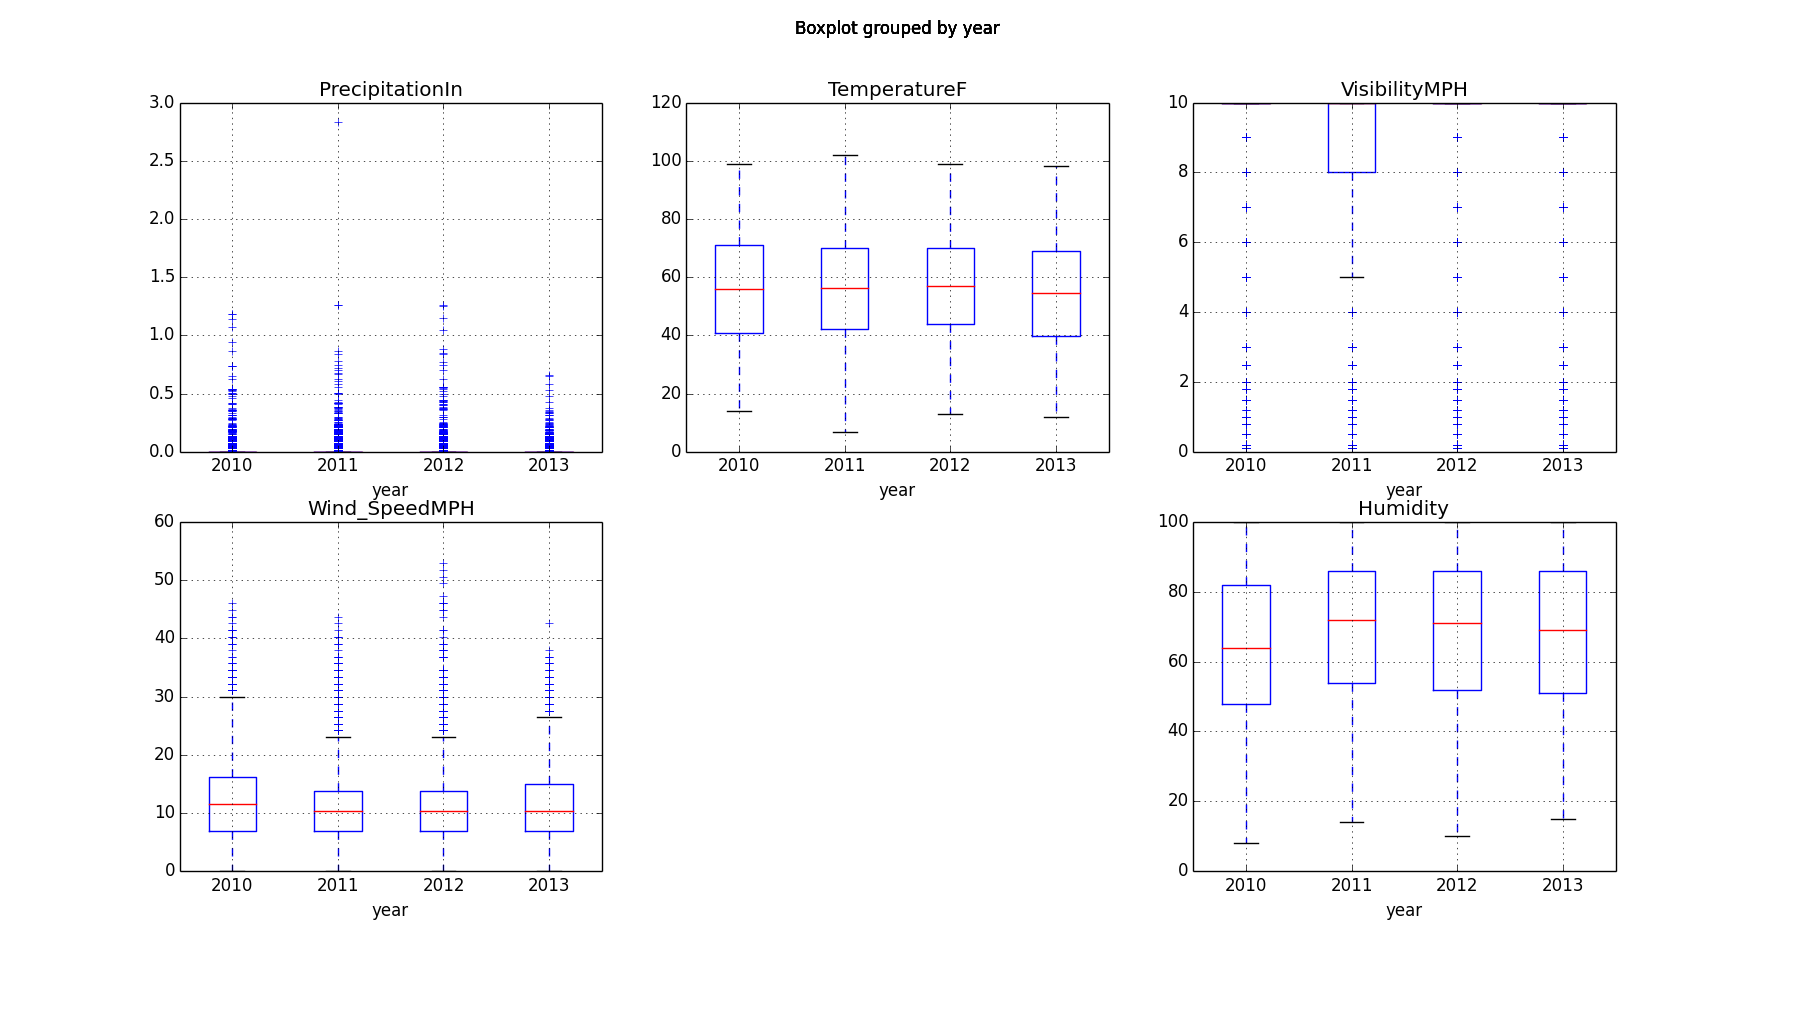
\includegraphics[scale=0.35]{./figures/boxplot_annualvariation.png}

\caption{JFK - annual exploratory statistics of METAR data}
\label{default}
\end{center}
\end{figure}


\section*{Conclusion}
In conclusion,
%%--LaTeX then BibTeX then LaTeX-%%%

\bibliographystyle{abbrv}
\bibliography{all}
\end{document} 